\documentclass{article}

\usepackage{graphicx}
\usepackage[hidelinks]{hyperref}
\usepackage{geometry}
\usepackage{amsmath}
\usepackage{listings}
\usepackage{wrapfig}
\usepackage{subcaption}
\usepackage{tikz}
\usetikzlibrary{positioning}

\geometry{
 a4paper,
 left=20mm,
 right=20mm,
 top=20mm,
 bottom=25mm,
}

\begin{document}

\begin{titlepage}
\begin{center}
\vspace*{1cm}
            
\Huge
\textbf{Final Project}
            
\vspace{1cm}

\Large
\text{Due: Thursday, December 12, 2024}

\vspace{2cm}

\text{\texttt{Brian High}} \\
\text{\texttt{Thomas Hynes}} \\
\text{\texttt{Jeremy Middleman}} \\
\text{\texttt{Andrei Phelps}} \\
\text{\texttt{Wayne Rudnick}} \\

\vspace{2cm}

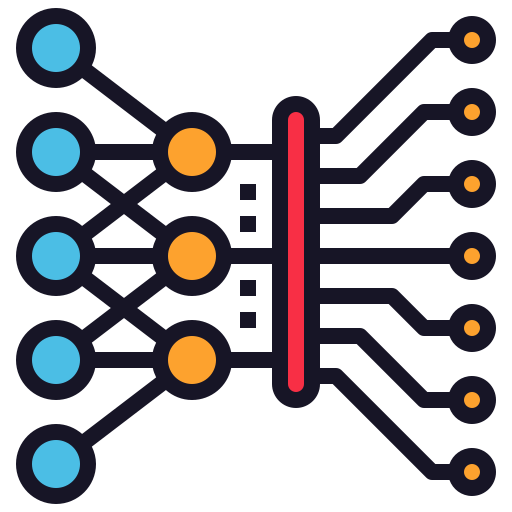
\includegraphics[scale=0.25]{figs/icon.png}\\[0.5cm]

\vspace{9cm}

\textbf{CS 491/591: Neural Networks} \\

\end{center}
\end{titlepage}

\section{Code Execution}

To execute the neural network training code, use the following command:
\begin{verbatim}
    python3 main.py
\end{verbatim}

You will need some packages which you might have to install separate. A requirements file was included. The code will run some tests by default, you can opt into these tests as well as change parameters like number of epochs at the top of main.

\section{Implementation of Convolution Neural Network}

\begin{figure}[!h]
    \centering
    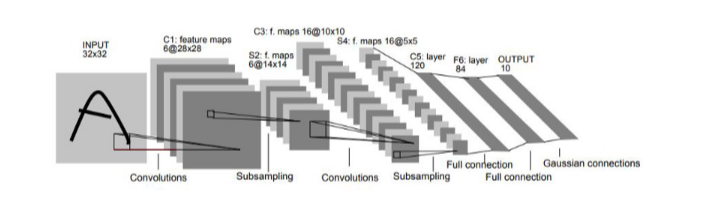
\includegraphics[width=0.75\linewidth]{figs/Capture.PNG}
\end{figure}

In our implementation of the CNN, we wanted to make sure that we were following the direction on the document, as well as using the helpful images that were provided to us.

In our implementation, we used three different layer classes. We had convolutional layers (with ReLU activations), pooling
layers (max pooling), and a fully connected layer class. With these classes, we build a sort of "chain" of layers in order to make the LeNet-5 structure. As per the document, we had: two convolutional layers (with ReLU activations), two pooling
layers (max pooling), and a fully connected (FC) neural network which has two hidden layers and one output layer. 

Our layers were able to complete forward and backward propagation. The layers differed from one another in their storage, (conv layer stored filters and FCL stored weights for example). They also differed in how they updated their "weights".



In our "chain" of layers, we compute values from one layer, and then pass the "weights" to the next layer. By using the carefully crafted LeNet-5, we are taking advantage of the smart design that was already devised to yield very strong machine learning results.

We think that while our implementation is good and allowed for us to get good results with training, that there are of course areas of potential improvement regarding optimization. We would like to reduce memory usage as well as reduce the number of loops we are performing overall. We are doing a ton of memory grabbing in these particular testing operations.

\subsubsection*{Description of classes (all contained within the same file)}
The ConvolutionalLayer performs the convolution using filters in self.filters which contains the filters/kernels used in the convolution and the filters' corresponding biases in self.biases. It includes the following methods: dataPadding for adding padding to the input data, forward to apply convolution and ReLU activation, and backward to compute gradients for backpropagation and update the filters and biases. 

The MaxPoolingLayer class does max-pooling with defined pool size and stride. This class finds the maximum value in each pass of the filter and stores it for the backward pass. The backward pass distributes gradients back in preparation for the next the forward pass.

The FullyConnectedLayer class calculates the weighted sum of the inputs coming from the convolution and pooling layers, applies ReLU, and computes the gradients for the weights, biases, and inputs during the backward pass. The LeNet5 class combines everything into the five layers. The forward method passes input data forward through the network, while backward propagates gradients back through the network. The filters, biases, and weights are updated using the update-params method.

\section{Optimizations}
We started this project by getting a working CNN. This implementation was rudimentary and slow, however we were able to verify that it worked. We found that using for loops to iterate through the multi-dimensional arrays was an easier way to understand and trouble shoot the CNN. We had a lot of trouble at first keeping the matrix operations in check, but using the for loops made the code more human readable. After a working implementation was achieved we needed to optimize the code to make it run in a reasonable time. The clear optimization to make was to convert a lot of the for loops to vector operations using built in functions. Most of the run time was coming from the convolution layer that a lot of matrix operations. We were not able to convert every operation to a vector operation but the optimization was enough to make the run in a reasonable time. 
\section{Test Cases}
\subsection{MNIST}


\begin{figure}[!h]
    \centering
    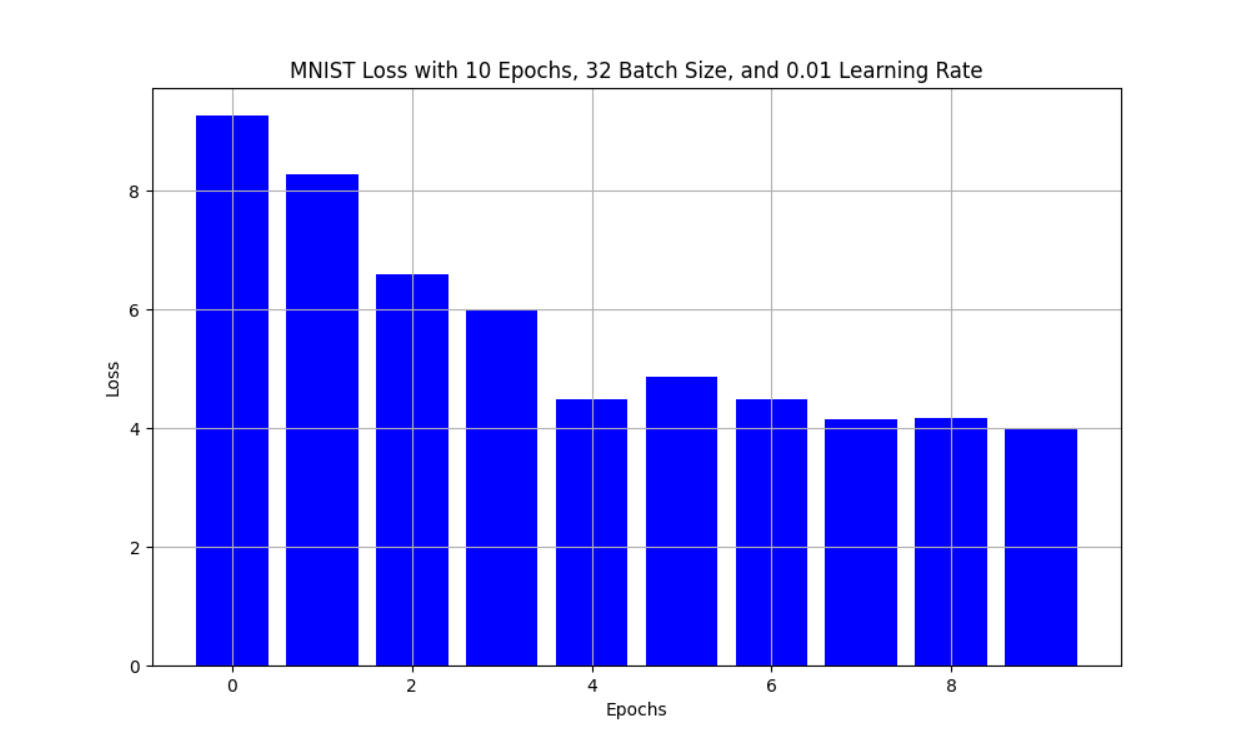
\includegraphics[width=0.75\linewidth]{figs/MNIST L 10-32-0.01.png}
\end{figure}

\begin{figure}[!h]
    \centering
    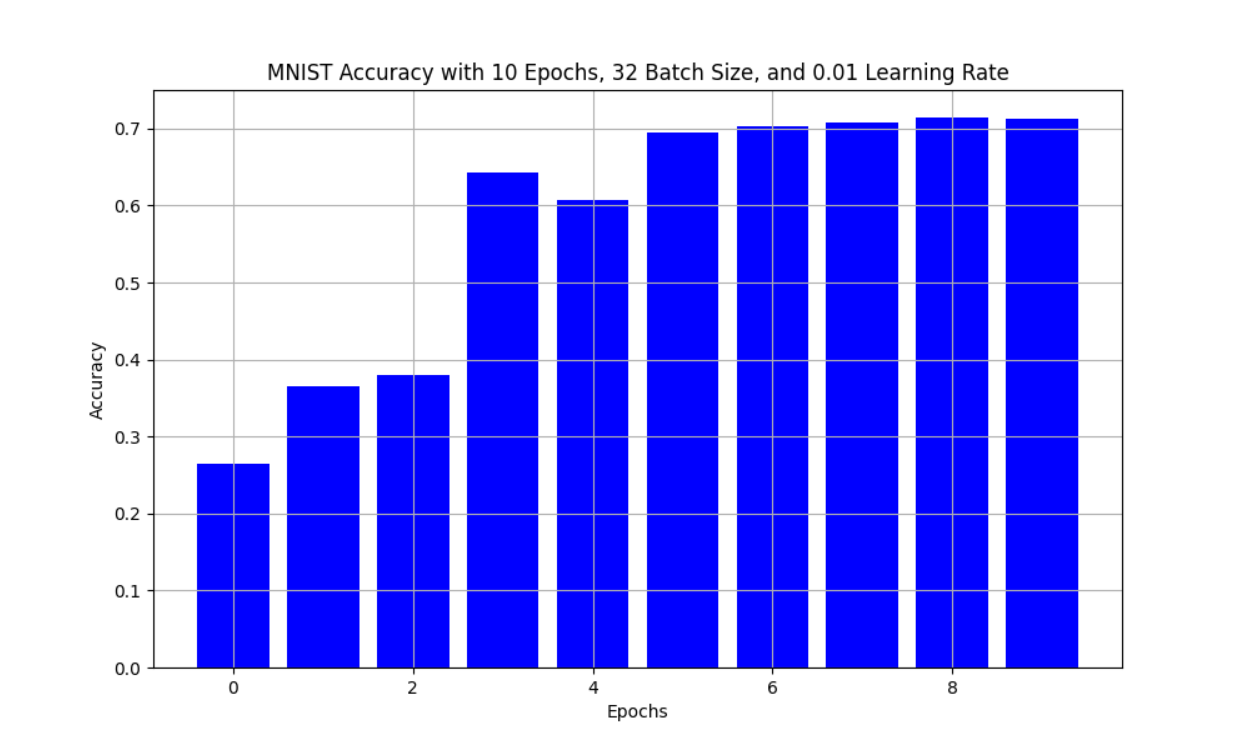
\includegraphics[width=0.75\linewidth]{figs/MNST A 10-32-0.01.png}
\end{figure}

\subsection{MNIST Results}

We found that our model actually performed quite well in regards to the MNIST testing. The way we set up our program allowed for a relatively seamless testing implementation here.

In our tests, which we plotted, it is easy to see that as the number of epochs increases, the loss goes down considerably whilst the accuracy goes up at the same time. This combination shows in a very strong way that our program was able to learn from the dataset and identify samples at a much higher rate than if it were simply guessing. We were all very impressed with this result, as we did not give the model a ton of time to learn (i.e. not a ton of iterations). Our group also felt that using this neural network for the MNIST was less viable than the FNN because of the overhead of this model. This model required more storage and took a lot more computation time and did not yield improvements in result when compared to the FNN. Using this model we had a more difficult time finding the correct parameters to be able to properly train our model on the MNIST data.

\begin{figure}[!h]
    \centering
    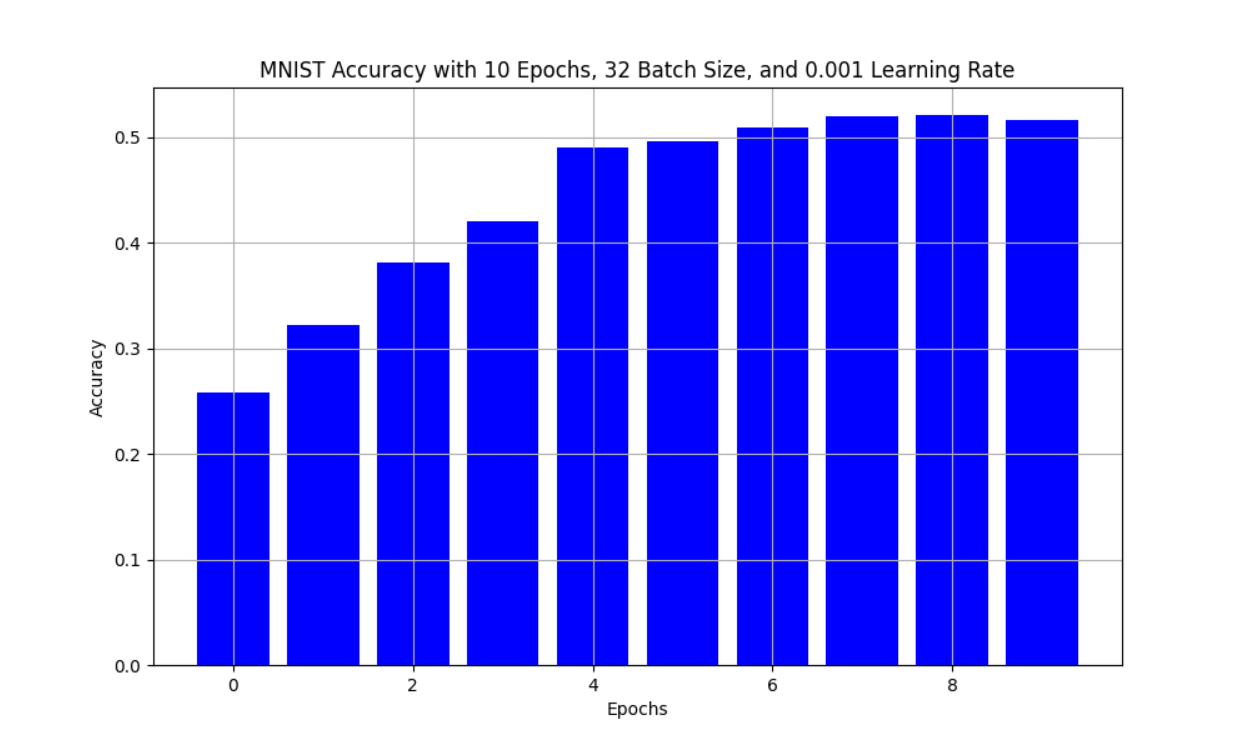
\includegraphics[width=0.75\linewidth]{figs/MNIST A 10-32-0.001.png}
\end{figure}

\subsection{CIFAR-10}

\begin{figure}[!h]
    \centering
    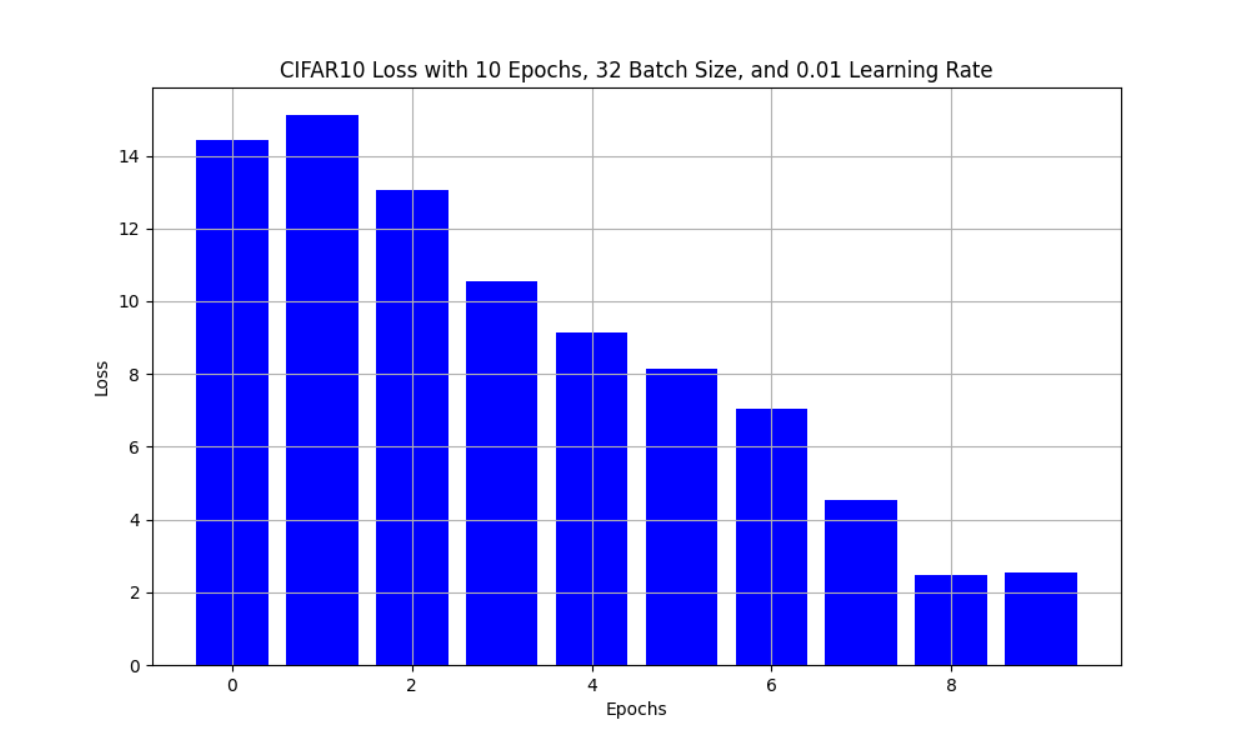
\includegraphics[width=0.75\linewidth]{figs/CIFAR L 10-32-0.01.png}
\end{figure}

\begin{figure}[!h]
    \centering
    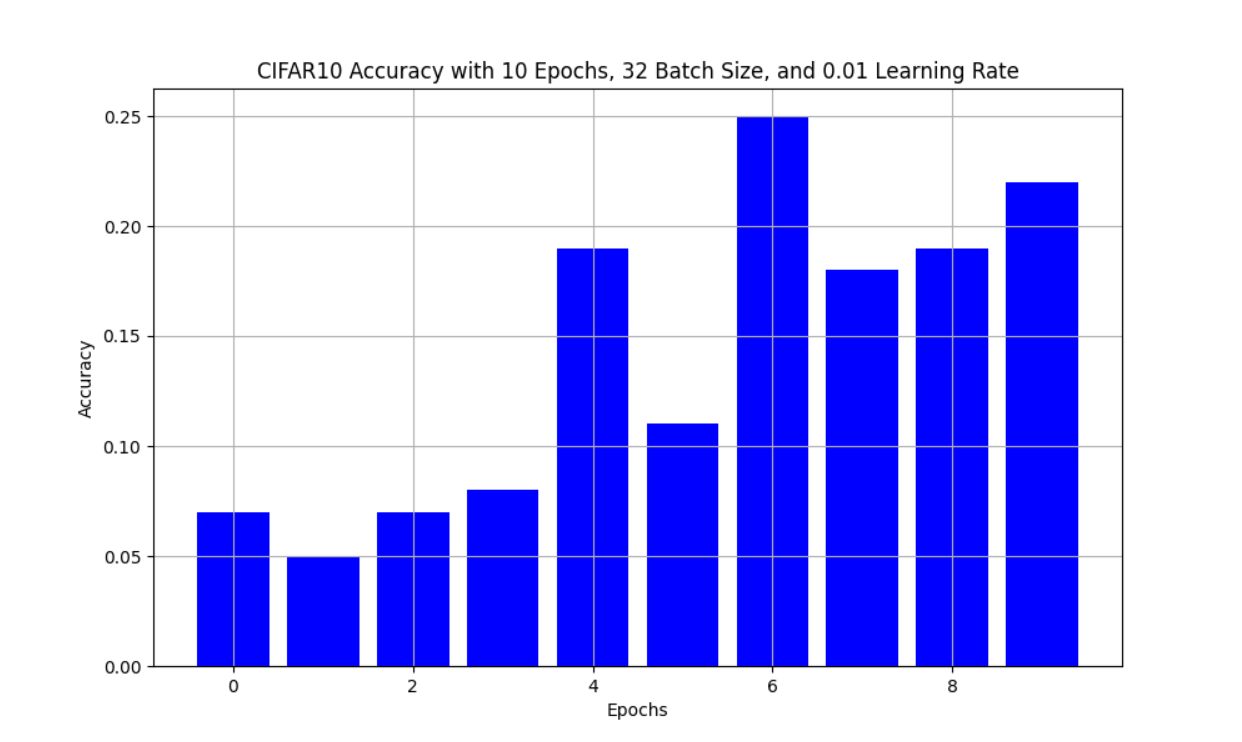
\includegraphics[width=0.75\linewidth]{figs/CIFAR A 10-32-0.01.png}
\end{figure}

\begin{figure}[!h]
    \centering
    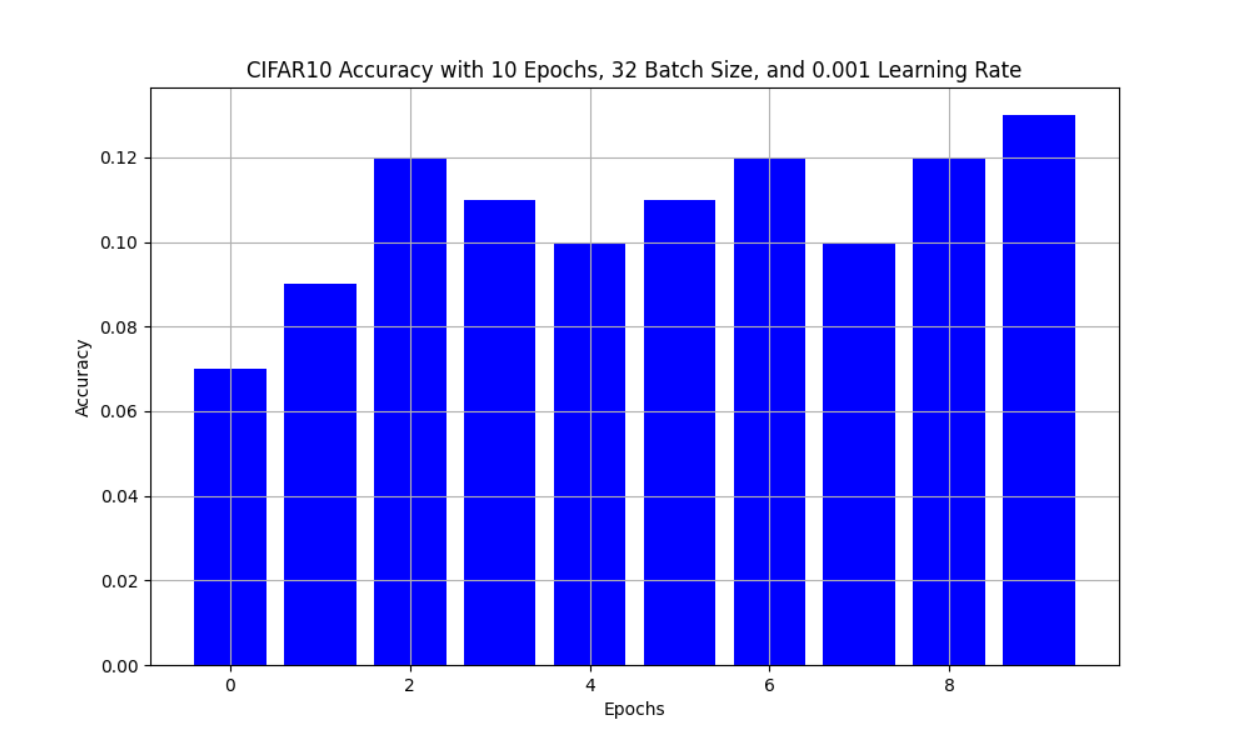
\includegraphics[width=0.75\linewidth]{figs/CIFAR A 10-32-0.001.png}
\end{figure}

\subsection{CIFAR-10 Results}
When it comes to machine learning, it is important to look at any rate which is above guessing to be a success in some way. In our case here, while our accuracy wasn't very high, we were able to see a massive improvement in the 0.01 learning rate test for instance. The CIFAR-10 dataset was not able to achieve the same accuracy that we were able to reach testing on MNIST, likely due to its higher complexity. Training 10 epochs with a learning rate of 0.01 took 10 minutes and 23 seconds. We had a guess rate of approximately 0.07 at epoch 0-2 and by epoch 10, we were almost at 0.25. That is a massive improvement with very few epochs overall.

We as a group think that this is a very positive result. Without any doubt, our model was able to correctly learn and identify the samples at a higher and higher rate as it learned. We are almost certain, that if we had more time to run the training, that we could see some very high accuracies with this model. The main limiting factor here for us was time. We plan to expand on this work and see just how much better this model can get when we give it something more like 100+ epochs to train on.

\newpage
\section{Proofs}

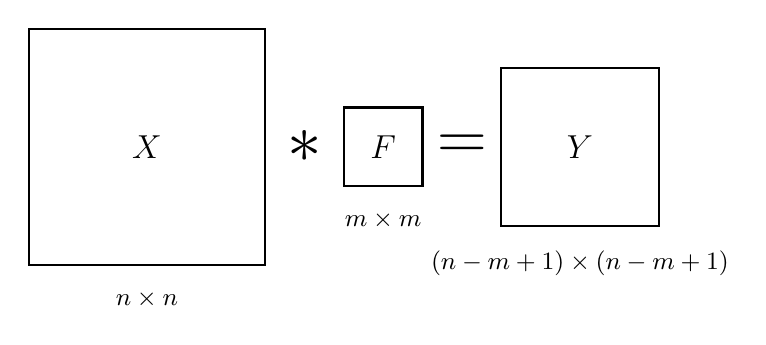
\begin{tikzpicture}
    % First (largest) square
    \draw[thick] (0, 0) rectangle (3, 3);
    \node at (1.5, 1.5) {\large $X$};

    % Convolves symbol
    \node at (3.5, 1.5) {\Huge $\ast$};

    % Second (smallest) square
    \draw[thick] (4, 1) rectangle (5, 2);
    \node at (4.5, 1.5) {\large $F$};

    % Equals symbol
    \node at (5.5, 1.5) {\Huge $=$};

    % Third (slightly smaller than first) square
    \draw[thick] (6, 0.5) rectangle (8, 2.5);
    \node at (7, 1.5) {\large $Y$};

    % Labels for sizes
    \node[anchor=north] at (1.5, -0.2) {\small $n \times n$};
    \node[anchor=north] at (4.5, 0.8) {\small $m \times m$};
    \node[anchor=north] at (7, 0.3) {\small $(n-m+1) \times (n-m+1)$};
\end{tikzpicture}

One note: as \( k \) is the depth of all three matrices, it is not shown in these calculations for simplicity.

As is seen in the picture, the \( X \) matrix containing the data has dimensions \( n \times n \), the filter has dimensions \( m \times m \), and the output \( Y \) matrix has dimensions \( (n - m + 1) \times (n - m + 1) \).

\subsection*{a}

\subsubsection{Analysis of the problem}

As shown in the formula below, when you take the derivative of the loss function with respect to \( Y \) and convolve that with \( X \), you get the derivative of the loss function with respect to \( F \):
\[
\frac{\partial \mathcal{L}}{\partial Y} \ast X = \frac{\partial \mathcal{L}}{\partial F}
\]

In this first proof, the following are being convolved: 
\begin{enumerate}
    \item the gradient of the loss function with respect to the output \( Y \), 
    \item the dataset \( X \).
\end{enumerate}

As a result of the alignment of subsections of \( X \) with the gradient of the loss function with respect to \( Y \), this convolution will necessarily form a matrix of size \( m \times m \), the same dimensions as the filter \( F \).

\subsubsection{Mathematical Proof}

\textbf{Definition:} The gradient of the loss function with respect to \( F \) is:
\[
\frac{\partial \mathcal{L}}{\partial F} = \left( \frac{\partial \mathcal{L}}{\partial Y} \cdot \frac{\partial Y}{\partial F} \right)
\]

for each of the k layers.

Statement of the gradient:

\[
Y = X \ast F
\]

The derivative of \( Y \) with respect to \( F \) is:
\[
\frac{\partial Y}{\partial F} = X.
\]

Apply chain rule substitution, which once again applies to each of the k layers:
\[
\frac{\partial \mathcal{L}}{\partial F} = \left( \frac{\partial \mathcal{L}}{\partial Y} \ast X \right).
\]

In order for this convolution above to take place, there needs to be padding of \( m - 1 \) to ensure the resulting dimensions match \( F \), which is \( m \times m\), and also applies to each of the k layers.

Thus, our original statement holds: the size of the gradient of the loss function with respect to \( F \) always has the same size as the filter \( F \).

\subsection{b}

\subsubsection{Analysis of the problem}

As shown in the formula below, when you take the derivative of the loss function with respect to \( Y \) and convolve that with \( F \), you get the derivative of the loss function with respect to \( X \):
\[
\frac{\partial \mathcal{L}}{\partial Y} \ast F = \frac{\partial \mathcal{L}}{\partial X}
\]

In this second proof, the following are being convolved: 
\begin{enumerate}
    \item the gradient of the loss function with respect to the output \( Y \), 
    \item the filter \( F \).
\end{enumerate}

As a result of the alignment of the filter \( F \) with the gradient of the loss function with respect to \( Y \), this convolution will necessarily form a matrix of size \( n \times n \), the same dimensions as the dataset \( X \).

\subsubsection*{Mathematical Proof}

\textbf{Definition:} The gradient of the loss function with respect to \( X \) is:
\[
\frac{\partial \mathcal{L}}{\partial X} = \left( \frac{\partial \mathcal{L}}{\partial Y} \cdot \frac{\partial Y}{\partial X} \right)
\]

for each layer.

Statement of the gradient:

\[
Y = X \ast F
\]

The derivative of \( Y \) with respect to \( X \) is:
\[
\frac{\partial Y}{\partial X} = F.
\]

Apply chain rule substitution, which once again applies to each layer.
\[
\frac{\partial \mathcal{L}}{\partial X} = \left( \frac{\partial \mathcal{L}}{\partial Y} \ast F \right).
\]

In order for this convolution above to take place, there needs to be padding of \( m - 1 \) to ensure the resulting dimensions match \( X \), which is \( n \times n \), and also applies to each layer.

Thus, our original statement holds: the size of the gradient of the loss function with respect to \( X \) for each of the k layers always has the same size as the dataset \( X \).

\section{Individual Contributions}

\subsection{Brian High}
\begin{itemize}
    \item[1)] Worked on the testing and training loop portion 
    \item[2)] Spent a lot of time diving into the CNN it optimize the run to be somewhat reasonable 
    \item[3)] Worked with all group memebers on the document
\end{itemize}

\subsection{Thomas Hynes}
\begin{itemize}
    \item[1)] Wrote the code to generate the graphs and ran the tests to get figures for MNIST and CIFAR datasets.
    \item[2)] Worked on and wrote sections in section 4 of our document. Helped with rest of group edit and correct any errors in the other sections of our document.
    \item[3)] Worked on code improving forward and backwards propagation methods in an effort to reduce computation time.
\end{itemize}

\subsection{Jeremy Middleman}
\begin{itemize}
    \item[1)] Wrote the proofs.
    \item[2)] As part of testing: wrote the part of main involved with loading the datasets and prepping them for running in the LeNet (i.e. everything but the actual running of LeNet and making the plots). Also edited the section where they are actually run.
    \item [3)] Also part of testing: helped identify optimal hyperparameters (reduced-data-size epochs) used in the CNN.
    \item [4)] Wrote "Description of classes" section as part of the description of the data structure of the CNN.
\end{itemize}

\subsection{Andrei Phelps}
\begin{itemize}
\item[1)] Implemented a backpropagation function for an individual convolutional layer.
\item[2)] Developed a backpropagation function for a single max pooling layer.
\item[3)] Worked with the team on the document.
\end{itemize}

\subsection{Wayne Rudnick}
\begin{itemize}
    \item[1)] Made a constructor which creates a CNN according to the given structure. Specified the CNN structure
    \item[2)] Made a forward function which performs a forward propagation on the neural network.
    \item[3)] Created the data fields which explicitly define each layer as well as the activations in the neural network
    \item[4)] Worked with all group members to add results to this document. Wrote on the testing results as well as the implementation of the CNN.
\end{itemize}

\end{document}
